\chapter{联邦学习中的自适应本地差分机制}

\label{ch3}
对于数据驱动的深度学习模型而言,模型参数学习数据特征的同时也记录下了敏感信息。在规定的差分隐私预算下,如何减少模型的可用性损失是关键。受传统的数据查询思想的影响,将差分隐私部署于深度学习模型中,首先可能会尝试通过仅处理由训练过程产生的最终参数(例如最终判别置信度等)来保护训练数据的私密性。这种方法将训练过程本身过程视为黑盒,但是深度学习的输出结果是一种高度抽象化的判别,细微的扰动就可能造成较大的差别。和数据隐私紧密相关的是训练过程中的梯度参数,因此针对梯度下降过程进行扰动,或将成为一种有效的保护方式。 

与传统的集中式深度学习相比,联邦学习通过分布式训练在一定程度上缓解了隐私泄漏的问题。然而,许多研究表明,攻击者仍然可以通过模型训练的梯度损害用户的隐私[13]。文献[20]表明,深度学习技术可以"记忆"模型中的训练数据信息。在这种情况下,敌方一旦通过白盒推理攻击或者黑盒推理攻击访问模型,就可以推演出客户端本地的训练数据。

中心化差分隐私[文献]是定义在相邻数据集上的,意味着需要一个可信的第三方来收集所有客户端的数据,进行隐私化处理。然而,在实际生活中想找到一个真正可信的第三方数据收集平台十分困难,这极大地限制了中心化差分隐私的应用。

后来的研究者们又在中心化差分隐私的基础上提出了本地化差分隐私,基于不可信第三方的前提下,其将数据隐私化的工作转移到每个用户,用户自己来处理和保护个人数据,极大地降低了隐私泄露的可能性。假设在联邦学习模型中有n个客户端,本地差分隐私定义在客户端层面,保证客户端的任意两条数据上得到类似的输出。本地化差分隐私的定理如下:
\begin{equation}\label{eq:本地差分隐私}

\end{equation}

本地化差分隐私继承了中心化差分隐私的串行和并行组合特性,但是两者所采用的噪声机制有所不同。中心化差分隐私的噪声机制主要以拉普拉斯机制和指数机制为主;本地化差分隐私的噪声机制主要以随机响应为主。

机器学习中模型的优化问题可以概括为ERM(最小经验风险)问题:
\begin{equation}\label{eq:ERM}
\arg \min _{\theta \in \mathcal{C}}\left(F(\theta):=\frac{1}{m} \sum_{i=1}^{m} F_{i}(\theta)\right)
\end{equation}

从隐私保护的角度讲,我们只要截断了从原始输入到输出,在其中加入一道隐私保护屏障,具体在哪一步截断则对应于不同的方法。差分隐私保护机器学习的方法具体有以下几种:
\begin{itemize}
	\item [\textbf{输入扰动:}] 输入扰动是在获取的训练数据上直接添加噪声,之后的模型训练和优化都是基于加躁后的训练数据。
	\item [\textbf{输出扰动:}] 输出扰动沿袭了拉普拉斯机制最简单的思路,即考虑函数输出的敏感度来添加噪声,那么在ERM公式中我们只需要考虑argmin函数输出的敏感度,基于这个敏感度来添加拉普拉斯噪声即可得到一个简单的满足差分隐私的ERM方法。
	\item [\textbf{梯度扰动:}] 梯度扰动是在执行最小化损失函数的过程中,设计满足差分隐私的算法。
	\item [\textbf{目标扰动:}] 目标扰动是在模型的目标函数中添加一个随机量,以使得最终模型的输出满足随机性。
\end{itemize}

基于梯度加噪的差分隐私保护方法作为主流的差分隐私应用于深度学习模型的方法之一,方案目标为满足差分隐私条件下实现最优的模型可用性。本章节主要从以下三个方面展开研究:首先,在模型中的不同层次采用不同的梯度裁剪阈值。梯度裁剪阈值作为一个重要的参数,既影响了有效的梯度学习过程,又作为数据敏感度成为噪声添加的参数之一,区别化的梯度裁剪手段将更大限度上保留了模型的可用性。其次,分析了梯度裁剪带来的敏感度变化,结合 MA 机制进行隐私预算的跟踪,使得整体隐私损失计量更加精确化,为模型训练预留更多的空间。最后,为了从实验上证实该方法的有效性,结合成员推理攻击进行验证,进一步证实了梯度自适应加噪模型在理论约束和实际表现中具有双重隐私可靠性。 


\section{攻击模型}
最近研究表明深度神经网络容易受到对抗样本的攻击。为了解决这个问题,一些工作通过向图像中添加高斯噪声来训练网络,从而提高网络防御对抗样本的能力,但是该方法在添加噪声时并没有考虑到神经网络对图像中不同区域的敏感性是不同的。针对这一问题,提出了梯度指导噪声添加的对抗训练算法。该算法在训练网络时,根据图像中不同区域的敏感性向其添加自适应的噪声,在敏感性较大的区域上添加较大的噪声,抑制网络对图像变化的敏感程度,在敏感性较小的区域上添加较小的噪声,提高其分类精度。
提出一种基于数据差分隐私保护的随机梯度下降算法。引入范数剪切与附加高斯噪声操作,对传统梯度更新策略进行改进。为衡量每次迭代过程中对数据隐私性的破坏,提出隐私损失累积函数在迭代过程中对数据隐私性的侵犯程度进行度量。

我们认为云服务器是一个 "诚实但好奇 "的实体。也就是说,服务器将遵循与所有用户的协议。然而,通过利用完全访问用户梯度的便利,它也试图在训练过程中获得关于客户端的额外的信息。出于这个原因,我们的提出的自适应加噪机制目的是保护发送到服务器的本地梯度不被推断出任何关于用户的额外信息,并且尽量维持原有模型的精度。


\section{模型概况}

\subsection{系统架构}

\begin{figure}[!hbt]
\centering
	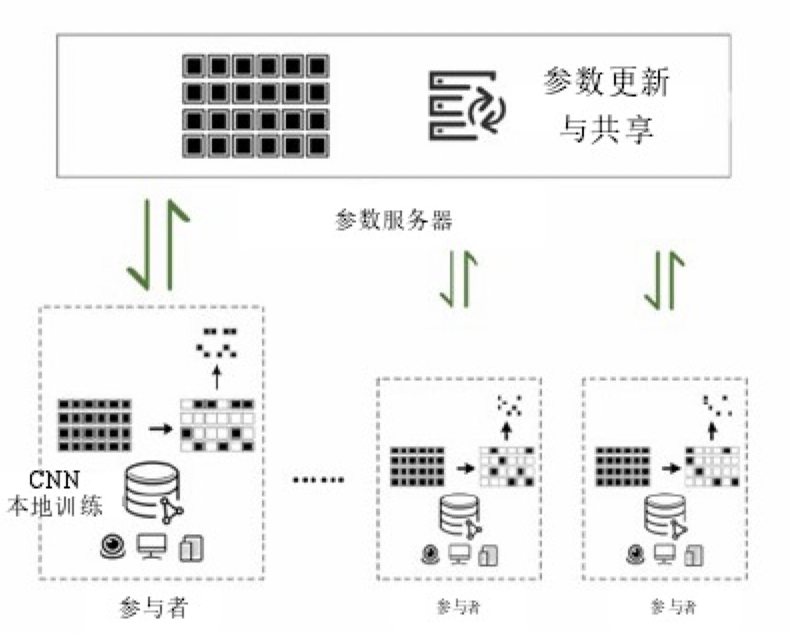
\includegraphics[scale=0.7]{fig2/C3/联邦学习系统架构}%联邦学习的系统架构
	\caption{联邦学习的系统架构}
	\label{fig:联邦学习的系统架构}	
\end{figure}

如图\ref{fig:联邦学习的系统架构}所示,在我们的系统模型中,有两方,即云服务器和用户。

\textbf{云服务器}:云服务器事先与用户协商一个网络框架。然后,服务器通过公共数据训练一个初始模型,然后将初始模型的参数广播给用户。用户在本地训练各自的模型后,云服务器收集用户发送的模型梯度,并更新全球模型。

\textbf{用户}:用户下载由云服务器初始化的模型参数。然后,每个用户在本地数据集上训练私人模型。最后,用户将本地模型的扰动梯度发送到云服务器。

每个参与者在第一次进入联邦学习系统时,都会初始化参数。针对统一的学习目标,在本地训练集上进行模型的训练。联邦学习系统同样包括参数交换协议,在参数交换协议下,参与者将本地所得神经网络梯度的参数上传至参数服务器,同样通过参数服务器下载最新的全局参数值至本地继续训练。参与者可以在本地独立训练时,避免了使用局限训练集的单个本地模型的过拟合。模型经过训练之后,每个参与者都可以使用新的测试集独立且隐私的对其进行评估与测试,无需再进行交互操作。 

\subsection{本地训练}
在分布式联邦学习中, 第 $i$ 个参与者在本地将会对全局神经网络参数的一个局部向量 $w^{i}$进行维护、学习和更新称之为本地训练。参数服务器负责对全局参数向量 $w^{g l o b a l}$进行维护和更新。每个参与者在开始训练时可以随机初始化本地参数, 也可以从参数服务器下载其参数最新值。

每个参与者都会使用统一标准的神经网络算法训练模型,使用的神经网络算法不局限于简单深度神经网络与卷积深度神经网络,但所有参与者需要进行统一, 本文使用的是采用选择性随机梯度下降算法全连接层的卷积神经网络 $\mathrm{CNN}$ 。 本地模型网络多次迭代训练其本地训练集。在本地训练期间,不同参与者之间不需要额外的共享样本和交互,他们通过参数服务器通过参数共享间接影响彼此的训练结果。

\begin{algorithm}[!htb]
	\caption{联邦学习客户端本地训练算法}
	\label{FLLT algorithm}
	\begin{algorithmic}[1]
		\footnotesize
		\STATE \textbf{Input:} 全局模型参数 $\boldsymbol{w}^{\text {global }}$, 初始化参数 $\boldsymbol{w}^{i}$
	    \STATE 参数服务器初始化模型
	    \STATE for $(epoch=1$ to $\mathrm{n})$ do
	    \STATE 从中央服务器下载全局参数 $\boldsymbol{\theta}_{d}$
	    \STATE 本地客户端在本地数据集上训练 $\boldsymbol{CNN}$模型
	    \STATE 根据步骤$(2-5)$更新$\boldsymbol{w}^{i}$ 
	    \STATE 计算梯度向量$\Delta \boldsymbol{w}^{i}$
		\STATE 将本地客户端的模型输出$\Delta \boldsymbol{w}_{s}^{i}$上传给参数服务器
		\STATE 结束训练
	\end{algorithmic}
\end{algorithm}

算法\ref{FLLT algorithm}描述了参与者在进行本地训练时具体步骤。每个参与者独立进行深度神学习训练,在每个训练阶段由五个步骤组成。在初始化之后, 第 $i$个参与者从参数服务器(Parameter Server, PS)中下载了最新参数的分量 $\theta_{d}$,将下载的值覆盖至其本地参数,之后会在本地训练数据集上训练神经网络。

在算法的第 6 步中,参与者计算全连接层算法训练局部参数变化得到梯度向量 $\Delta w^{i}$ 。参数 $\Delta w^{i}$ 反映了对于第 $i$ 个参与者, 每个神经元中的权重向量需要变化多少能够 得到更精确的模型。 $\Delta w^{i}$的参数信息正是其他参与者需要训练更好模型以及避免的本地数据过拟合的信息。
$\Delta \boldsymbol{w}_{s}^{i}$ 表示经过选择后上传的参数。在上传训练结果前,选择一个大于阈值 $T$ 的子 集替代完整的参数向量, 参与者选择上传更有助于目标函数的梯度值, 可以使得训练迭代过程收敛更快, 模型精度更高, 以及陷入局部最优的可能性更小。

在本地训练时,卷积神经网络的全连接层采用了选择性随机梯度下降算法。Shokri在\upcite{ref35}中证明了其与传统的随机梯度下降算法有着几乎相同的准确性。原因是选择参数上传更新全局模型与传统随机梯度下降算法求最优值的原因相同,选择的过程增加了最优化过程的随机性。

参与者单独训练模型时, 由于训练集的多次使用与缺少更新, 很容易陷入局部最优。在训练本地模型时,参与者使用梯度参数的子集对模型进行更新, 会增加模型优化过程中的随机性, 很大程度上避免了本地$\mathrm{SGD}$过多使用相同的小样本集产生的模型过拟合。使用其他参与者用在不同数据集上训练学习的值覆盖本地学习的参数,可以邦助每个参与者跳出局部最优,从而得到更准确的模型。

\subsection{全局参数更新}
联邦学习通过协调深度学习任务, 建立统一的深度学习模型结构后, 参数服务器会初始化全局参数 $w^{gloabal}$。之后处理系统内参与者的上传和下载请求, 存储参与者的局部参数, 并计算更新全局参数 $w^{g l o b a l}$。当参与者上传参数时,参数服务器会将上传的 $\Delta\boldsymbol{w}_{s}^{i}$的值添加至相应的全局参数中,并为每个全局权重参数更新元数据和计数器stat。具体更新规则如下:

对于所有的 $j \in S$ :
\begin{equation}\label{eq:全局参数更新1}
w^{\text {global }}:=w^{\text {global }}+\Delta \boldsymbol{w}_{j}^{i}
\end{equation}


为了增加更新的参数的权重, 服务器可以周期性地将计数器乘以衰减因子 $\beta$, 即:
\begin{equation}\label{eq:全局参数更新2}
\text { stat }:=\beta \cdot \text { stat }
\end{equation}
当参与者从服务器获取具有最大统计值参数的最新值时, 将在下载期间使用这些统计信息。每个参与者都可以通过设置 $\theta_{d}$决定下载这些参数的某一部分。

\section{方案设计}{}
\subsection{层间依赖传播算法}
如图\ref{fig:层间依赖传播算法}每个用户在本地用原始数据进行训练,在神经网络中进行前向传播操作,得到本地模型的输出。

\begin{figure}[!hbt]
\centering
	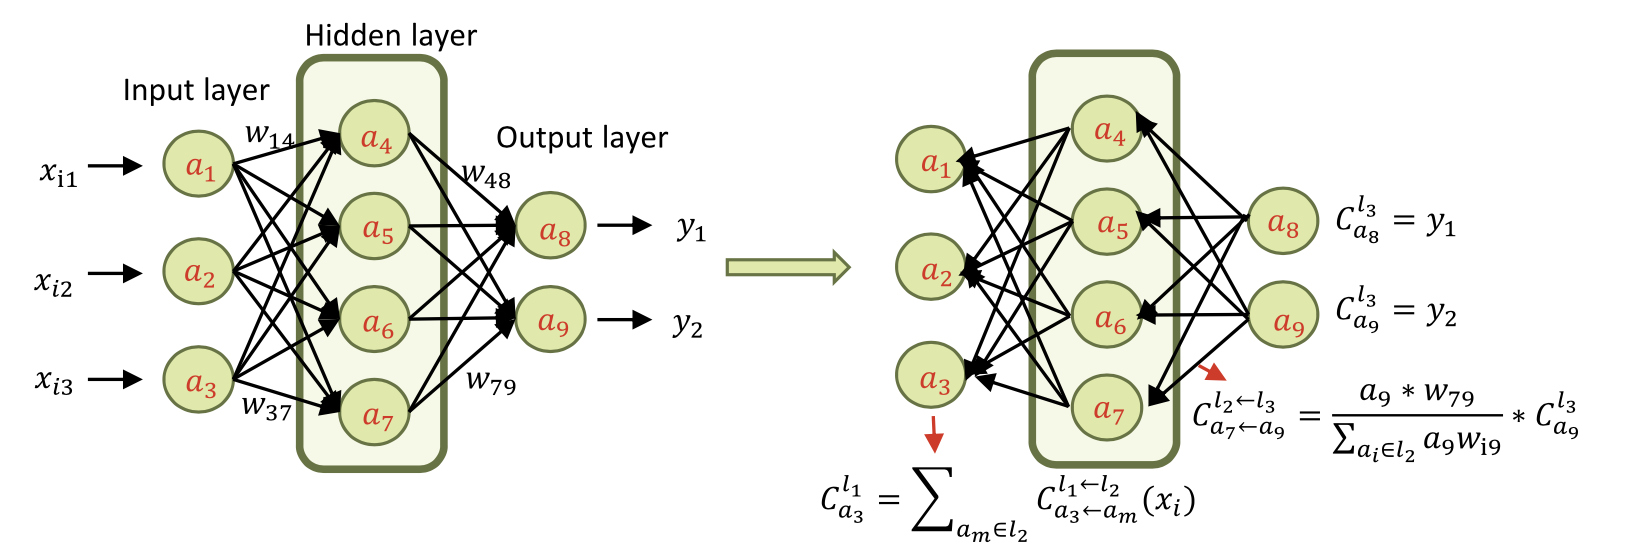
\includegraphics[scale=0.5]{fig2/C3/前向传播算法}%联邦学习的系统架构
	\caption{层间依赖传播算法}
	\label{fig:层间依赖传播算法}	
\end{figure}

根据矩阵层之间的线性相关性,神经元$a_{i}$在第k层的贡献$C_{a_{i}}^{l_{k}}\left(x_{i}\right)$等于连接到神经元$a_{i}$的相邻层的贡献之和:
\begin{equation}\label{eq:层间传播1}
C_{a_{i}}^{l_{k}}\left(x_{i}\right)=\sum_{a_{j} \in l_{k+1}} C_{a_{i} \leftarrow a_{j}}^{l_{k} \leftarrow l_{k+1}}\left(x_{i}\right)
\end{equation}

比如,在图\ref{fig:层间依赖传播算法}中,存在:
\begin{equation}\label{eq:层间传播2}
C_{a_{7}}^{l_{2}}\left(x_{i}\right)=\sum_{a_{j} \in l_{3}} C_{a_{7} \leftarrow a_{j}}^{l_{2} \leftarrow l_{3}}\left(x_{i}\right)=C_{a_{7} \leftarrow a_{8}}^{l_{2} \leftarrow l_{3}}\left(x_{i}\right)+C_{a_{7} \leftarrow a_{9}}^{l_{2} \leftarrow l_{3}}\left(x_{i}\right)
\end{equation}

其中,"←"表示两部分之间的连接关系。具体来说,"l2 ← l3 "是指深度神经网络(DNN)中第二次层和第三层之间相邻层的连接关系。那么对于第k个输出层:
\begin{equation}
C_{a_{i}}^{l_{k}}\left(x_{i}\right)=f\left(x_{i},\omega_{i}^{r}\right)
\end{equation}

因此,神经元$a_{j}$对于输出层的贡献等于模型的输出。第k层的神经元$a_{j}$对于第k-1层的神经元$C_{a_{i} \leftarrow a_{j}}^{l_{k-1} \leftarrow l_{k}}\left(x_{i}\right)$等于:
\begin{equation}
C_{a_{i} \leftarrow a_{j}}^{l_{k-1} \leftarrow l_{k}}\left(x_{i}\right)=\left\{\begin{array}{cc}\frac{a_{i} w_{i, j}}{\sum_{a_{i} \in l_{k-1} a_{i} w_{i, j}}} C_{a_{j}}^{l_{k}}\left(x_{i}\right) & \sum_{a_{i} \in l_{k-1}} a_{i} w_{i, j} \neq 0 \\ \mu & \sum_{a_{i} \in l_{k-1}} a_{i} w_{i, j}=0\end{array}\right.
\end{equation}

其中$\mu$是一个无限接近于零,但大于零的数字。从上述公式中,我们可以认为每一层的贡献是相等的,而且贡献是逐层传递的。根据以上公式的推导,我们能得到神经网络模型中每一层以及每个神经元的贡献值。


\subsection{自适应噪声添加}
该机制对连续数值型数据划分变换范围并进行分段,根据分段将其变换为 1 维二元分类数据。转换后使用随机响应机制进行扰动,再根据扰动后的数据标识的数值段从中随机均匀抽取数值作为扰动。在真实数据和合成数据中的均值估计实验结果表明该机制极大地提高了准确性。除此之外,将分类变换扰动机制用于构建满足本地差分隐私的小批量梯度下降算法,并完成线性回归学习任务,实验结果证明该方法同样优于其他已有机制,可得到更小的均方误差。

在第二章中介绍了关于神经网络的结构,
\begin{equation}\label{eq:神经网络参数传递}
y=a(\mathbf{x} * \omega+b)
\end{equation}

公式\ref{eq:神经网络参数传递}是学习模型中每个隐藏神经元的转化过程。
其中$\mathbf{x}$代表输入向量,$y$是输出,$b$和$\omega$分别代表偏置项和权重矩阵。$a()$是一个激活函数,用于结合线性变换和非线性变换。$y=a(\mathbf{x} * \omega+b)$ 是线性变换部分。

由于神经网络的结构,上一层的输出是下一层的输入,由此我们可以得出,原始数据只被第一隐层的线性变换所利用。直观地说,为了得到一个具有隐私保护的学习模型,我们可以在第一层隐藏层的数据中注入噪声。正如Phan等人\upcite{ref36}提到的,对于线性变换有一种传统的方法,即向原始数据注入具有相同隐私预算的噪声,但是这容易导致隐私预算增加,并且使原始数据失真过多。因此,本文提出一种自适应噪声添加算法,针对每个梯度计算其贡献值,根据贡献值进行梯度裁剪并添加噪声。

首先,引入了两个调整因素。其中,$f$代表一个阈值,用于决定属性对模型结果输出的贡献是高还是低,其值由用户定义,即贡献超过阈值$f$的属性类对输出的贡献更大。然后,我们向所有这些属性注入自适应拉普拉斯噪声。当贡献率低于阈值$f$时,对这些属性进行概率选择。也就是说,我们选择概率为$1-p$的原始数据,并对一些概率为$p$的属性注入自适应拉普拉斯噪声。该公式如下:
\begin{equation}\label{eq:神经网络加噪}
\tilde{x}_{i, j}=\left\{\begin{array}{ll}
\ddot{x}_{i, j} & \beta \geq f \\
\bar{x}_{i, j} & \beta<f
\end{array}\right.
\end{equation}

其中$\beta$代表贡献率:$\beta=\frac{\left|\ddot{C}_{j}\right|}{\sum_{j=1}^{u}\left|\ddot{C}_{j}\right|}$,当$\beta<f$时,我们有:
\begin{equation}\label{eq:神经网络加噪2}
\bar{x}_{i, j}=\left\{\begin{array}{l}
\ddot{x}_{i, j} \text { with probability } p \\
x_{i, j} \text { with probability } 1-p
\end{array}\right.
\end{equation}


$f$和$p$是超参数,用户可以根据自己的情况来调整。

也就是说,隐私预算$\epsilon_{l}$是根据贡献率:$\epsilon_{j}=\frac{u *\left|\ddot{C}_{j}\right|}{\sum_{j=1}^{u}\left|\ddot{C}_{j}\right|} * \epsilon_{l}$。按比例分配给每个属性类。自适应噪声按以下方式注入属性中:
\begin{equation}\label{eq:神经网络加噪3}
x_{i, j}^{\prime}=x_{i, j}+\frac{1}{\left|D_{i}^{t}\right|} \operatorname{Lap}\left(\frac{G S_{l}}{\epsilon_{j}}\right)
\end{equation}

在不丧失一般性的情况下,调整因子$f$和$p$的值与系统的准确性和隐私水平有关。即$f$越小,$p$越大。越高的秘密水平,准确性越低,反之亦然。

我们用层间相关性传播(LRP)算法将输出分解到每一层。关于LRP算法的更多细节,我们将在以下部分进行介绍。每个用户都在本地对原始数据进行训练前馈操作,这可以获得一个新的数据操作,从而获得本地模型的输出。根据相邻层之间的线性关系,在第k层的神经元的贡献$C_{a_{i}}^{l_{k}}\left(x_{i}\right)$等于连接到神经元$a_{i}$的相邻层的贡献之和:
\begin{equation}\label{eq:神经网络加噪4}
C_{a_{i}}^{l_{k}}\left(x_{i}\right)=\sum_{a_{j} \in l_{k+1}} C_{a_{i} \leftarrow a_{j}}^{l_{k} \leftarrow l_{k+1}}\left(x_{i}\right)
\end{equation}

例如图\ref{fig:层间依赖传播算法}所示,我们有:
\begin{equation}
C_{a_{7}}^{l_{2}}\left(x_{i}\right)=\sum_{a_{j} \in l_{3}} C_{a_{7} \leftarrow a_{j}}^{l_{2} \leftarrow l_{3}}\left(x_{i}\right)=C_{a_{7} \leftarrow a_{8}}^{l_{2} \leftarrow l_{3}}\left(x_{i}\right)+C_{a_{7} \leftarrow a_{9}}^{l_{2} \leftarrow l_{3}}\left(x_{i}\right)
\end{equation}

其中,"$\leftarrow$"表示两部分之间的连接关系。"$l_{2} \leftarrow l_{3}$" 是指深度神经网络(DNN)中$2-t h$层和第3层之间相邻层的连接关系。
当第k层为输出层时,我们有:
\begin{equation}
C_{a_{i}}^{l_{k}}\left(x_{i}\right)=f\left(x_{i}, \omega_{i}^{r}\right)
\end{equation}

\subsection{隐私性证明}
随机隐私保护调整技术对线性变换函数进行了扰动,该函数满足$\left(\epsilon_{c}+\epsilon_{l}\right)$差分隐私。证明如下。
假设两个相邻的批次$D_{i}^{t}$和$D_{i}^{t^{\prime}}$,其最后一个元组$x_{n}$和$x_{n}^{\prime}$不同,$z\left(D_{i}^{t}\right)$和$z\left(D_{i}^{t^{\prime}}\right)$分别为线性变换函数。

一般来说,我们把偏置项视为第一类数据属性,即:$x_{i,0}=b_{i}$。线性转换可以改写为:$\ddot{\mathbf{z}}_{x \in D_{i}^{t}}(\omega)=\ddot{\mathbf{x}} * \omega$。线性变换的敏感性$G S_{l}$如下:
\begin{equation}
\begin{aligned}
G S_{l} &=\sum_{a_{i} \in l_{1}} \sum_{j=1}^{u}\left\|\sum_{x_{i} \in D_{i}^{t}} x_{i, j}-\sum_{x_{i}^{\prime} \in D_{i}^{t^{\prime}}} x_{i, j}^{\prime}\right\|_{1} \\
&=\sum_{a_{i} \in l_{1}} \sum_{j=1}^{u}\left\|x_{n, j}-x_{n, j}^{\prime}\right\|_{1} \\
& \leq \sum_{a_{i} \in l_{1}} \sum_{j=1}^{u} \max _{x_{i} \in D_{i}^{t}}\left\|x_{n, j}\right\|_{1} \\
& \leq \sum_{a_{i} \in l_{1}} u
\end{aligned}
\end{equation}

其中,$a_{i} \in l_{1}$是指第一隐藏层$l_{1}$中的神经元$a_{i}$,$u$是数据元组$x_{i} \in D_{i}^{t}$中的属性数。它包括两个调整因素。$f$和$p$,它们可以过滤多余的噪声。之后的属性的一般表达式如下:
\begin{equation}
\begin{aligned}
\tilde{x}_{i, j} &=[(1-f)+f * p] * \ddot{x}_{i, j}+f *(1-p) * x_{i, j} \\
&=[(1-f)+f * p]\left[x_{i, j}+\operatorname{Lap}\left(\frac{G S_{l}}{\epsilon_{j}}\right)\right]+[f *(1-p)] x_{i, j} \\
&=x_{i, j}+[(1-f)+f * p]\left[\operatorname{Lap}\left(\frac{G S_{l}}{\epsilon_{j}}\right)\right]
\end{aligned}
\end{equation}
然后我们可以得到:

\begin{equation}
\begin{aligned}
\frac{\operatorname{Pr}\left(\ddot{\mathbf{z}}_{D_{i}^{t}}(\omega)\right)}{\operatorname{Pr}\left(\ddot{\mathbf{z}}_{D_{i}^{t}}(\omega)\right)} &=\frac{\prod_{a_{i} \in l_{1}} \prod_{j=1}^{u} \exp \left(\frac{\epsilon_{j}\left\|\sum_{x_{i} \in D_{i}^{t}} x_{i, j}-\sum_{x_{i} \in D_{i}^{t}} \tilde{x}_{i, j}\right\|_{1}}{G S_{l}}\right)}{\prod_{a_{i} \in l_{1}} \prod_{j=1}^{u} \exp \left(\frac{\epsilon_{j}\left\|\sum_{x_{i}^{\prime} \in D_{i}^{t^{\prime}}} x_{i, j}^{\prime}-\sum_{x_{i}^{\prime} \in D_{i}^{t^{\prime}}} \tilde{x}_{i, j}^{\prime}\right\|_{1}}{G S_{l}}\right)} \\
& \leq \prod_{a_{i} \in l_{1}} \prod_{j=0}^{u} \exp \left(\frac{\epsilon_{j}}{G S_{l}}\left\|\sum_{x_{i} \in D_{i}^{t}} x_{i, j}-\sum_{x_{i}^{\prime} \in D_{i}^{t^{\prime}}} x_{i, j}^{\prime}\right\|_{1}\right) \\
& \leq \prod_{a_{i} \in l_{1}} \prod_{j=0}^{u} \exp \left(\frac{\epsilon_{j}}{G S_{l}} \max _{x_{i} \in D_{i}^{t}}\left\|x_{n, j}\right\|_{1}\right) \\
& \leq \exp \left(\epsilon_{l} \frac{\sum_{a_{i} \in l_{1}} u\left[\sum_{j=1}^{u} \frac{\left|\ddot{C}_{j}\right|}{\sum_{j=1}^{u}\left|\ddot{C}_{j}\right|}\right]}{G S_{l}}\right) \\
&=\exp \left(\epsilon_{l}\right)
\end{aligned}
\end{equation}

根据上述推倒证明可知,在联邦学习的神经网络中添加自适应噪声后,所上传的梯度是满足$\left(\epsilon_{c}+\epsilon_{l}\right)$差分隐私的。在满足差分隐私的基础上,在下一节我们会给予隐私损失累积函数计算隐私成本。

\subsection{隐私预算分析}
对于所提差分隐私SGD算法,除了确保算法运行的准确率以外,另一个重要的问题就是评估算法训练时的数据隐私损失成本。为此,提出隐私损失累积函 数的概念来进行每次迭代过程访问训练数据的隐私损 失以及随着训练进展时的累积隐私损失。
为不失一般性,令 $\sigma=\frac{\sqrt{2 \log (1.25 / \delta)}}{\varepsilon}$, 文献[36]严格证明,对于抽样概率 $q=\frac{\mathcal{L}}{N}$ 且 $\varepsilon<1$, 则对于完整样本而言,每次迭代过程都是 $(O(q \varepsilon),q \varepsilon)$-差分隐私的。 但文献并末对迭代过程以及噪声强度对差分隐私损失的影响展开研究,故无法对噪声强度以及剪切阈值$C$进行有依据的选取。故首先需要研究迭代过程对差分隐私的影响机制。

事实上,若令 $\sigma \geqslant c_{2} \frac{q \sqrt{T \log (1 / \delta)}}{\varepsilon}$,则同样应用文献[36]方法,可以严格证明算法对于任意的 $\varepsilon<c_{1} q^{2} T$ 都是 $(O(q \varepsilon \sqrt{T}),\delta)-$ 差分隐私的,其中 $c_{1}$ 和 $c_{2}$ 为常数。与文献\upcite{ref36}相比,本文算法能够在相同迭代步骤下,大幅度降低 $\varepsilon$ 的数值,对数据的隐私性保护更高。进一步地, 对于两个相邻的数据集 $d$,$d^{\prime} \in D$ 和映射机制 $M$,引入一个辅助输入变量 aux和输出$o \in R$, 定义映射机制$M$在输出$o$处的隐私损失为:
\begin{equation}
c\left(o ; M, a u x, d, d^{\prime}\right) \triangleq \log \frac{\operatorname{Pr}[M(a u x, d)=o]}{\operatorname{Pr}\left[M\left(a u x, d^{\prime}\right)=o\right]}
\end{equation}

对于所提差分隐私SGD算法而言,神经网络各层权重系数的参数值与每次迭代过程中的差分隐私机制有着紧密的关联,从而对于给定的映射机制 $M$,在第 $\lambda$ 次迭代过程的隐私损失定义为:
\begin{equation}\label{eq:隐私损失定义}
\begin{array}{r}
\alpha_{\mathcal{M}}\left(\lambda ; a u x, d, d^{\prime}\right) \triangleq \log \mathbb{E}_{o \sim M(a u x, d)}[\exp (\lambda c(o) ; M \\
\left.\left.\left.d,d^{\prime}\right)\right)\right]
\end{array}
\end{equation}

进一步地,映射机制 $M$ 的损失边界值定义为:
\begin{equation}\label{eq:损失边界值定义}
\alpha_{\mathcal{M}}(\lambda) \triangleq \max _{a u x, d, d^{\prime}} \alpha_{M}\left(\lambda ; a u x, d, d^{\prime}\right)
\end{equation}

其满足以下特性:

\begin{itemize}
\item 组合特性:给定一个机制 $M$, 由一组子机制顺序 $\left\{M_{1}, M_{2}, \cdots, M_{k}\right\}$ 组成,并满足$M_{i}: \prod_{j=1}^{i-1} R_{j} \times D \rightarrow R_{i}$,从而总隐私损失边界满足:
\begin{equation}\label{eq:损失边界值定义2}
\alpha_{M}(\lambda) \leqslant \sum_{i=1}^{k} \alpha_{M_{i}}(\lambda)
\end{equation}

\item 差分隐私边界:$\forall \varepsilon>0$, 映射机制 $M$ 是 $(\varepsilon,\delta)$ 差分隐私的,当且仅当:
\begin{equation}\label{eq:损失边界值定义2}
\delta=\min _{\lambda} \exp \left(\alpha_{M}(\lambda)-\lambda \varepsilon\right)
\end{equation}
\end{itemize}

上述2条性质确定了深度神经网络算法每次迭代的隐私损失以及所能够达到侵犯数据隐私容忍度的最大迭代次数。特别地,在附加高斯噪声的情况下,不妨令 $\mu_{0}$,$\mu_{1}$ 分别为 $N\left(0,\sigma^{2}\right)$ 和 $N\left(0,\sigma^{2}\right)$ 的概率密度函数,而 $\mu$ 为两个高斯密度函数的混合概率密度函数,即$\mu=(1-q) \mu_{0}+q \mu_{1}$。依据式\ref{eq:隐私损失定义}-\ref{eq:损失边界值定义2}可推导得 $\alpha$ $(\lambda)=\log \max \left(E_{1},E_{2}\right)$, 其中:
\begin{equation}\label{eq:隐私容忍1}
E_{1}=\mathbb{E}_{z \sim \mu_{0}}\left[\left(\frac{\mu_{0}(z)}{\mu(z)}\right)^{\lambda}\right]
\end{equation}

\begin{equation}\label{eq:隐私{}容忍2}
E_{1}=\mathbb{E}_{z \sim \mu_{0}}\left[\left(\frac{\mu_{0}(z)}{\mu(z)}\right)^{\lambda}\right]
\end{equation}

\section{本章总结}
联邦学习以分布式学习技术为基础,使参与者彼此通过一定的方式(如中心服务器)联合起来训练一个神经网络。在这个过程中,参与者不需要将自己的隐私数据暴露出来便可以参与协作训练,可以克服参与者本地数据集较小、数据样本比较单一、隐私泄露等缺点。虽然基本的分布式协作深度学习没有直接暴露参与者的隐私数据集,但是恶意攻击者仍然可以通过共享的参数等信息获得一定的隐私信息。 

本章详细介绍了基于梯度自适应加噪的差分隐私保护模型对于模型准确度的影响。其中梯度下降作为一种常见的深度学习优化方法,将梯度进行噪声扰动是最早被提出、也是目前相对主流的差分隐私加噪方案之一。通过将梯度裁剪的阈值根据网络层次进行适应性调整,能够使得噪声的添加造成的模型可用性损失更小,结合MA机制进行隐私预算的细化分配,实验表现为相比较固定梯度裁剪阈值而言,模型准确率更高。而且利用深度学习中的成员推理攻击证明梯度自适应加噪的方法在实验表现上也是有效的。然而,客户端的匿名性不足以防止侧信道链接攻击,例如,如果客户端在每次迭代中同时上传了大量的权重更新,云仍然可以将它们链接在一起。因此下一章将针对一种训练轮数无关的安全聚合模型进行研究。

